\begin{figure}[p]
\centering
    \begin{subfigure}[t]{\textwidth}
        \centering
    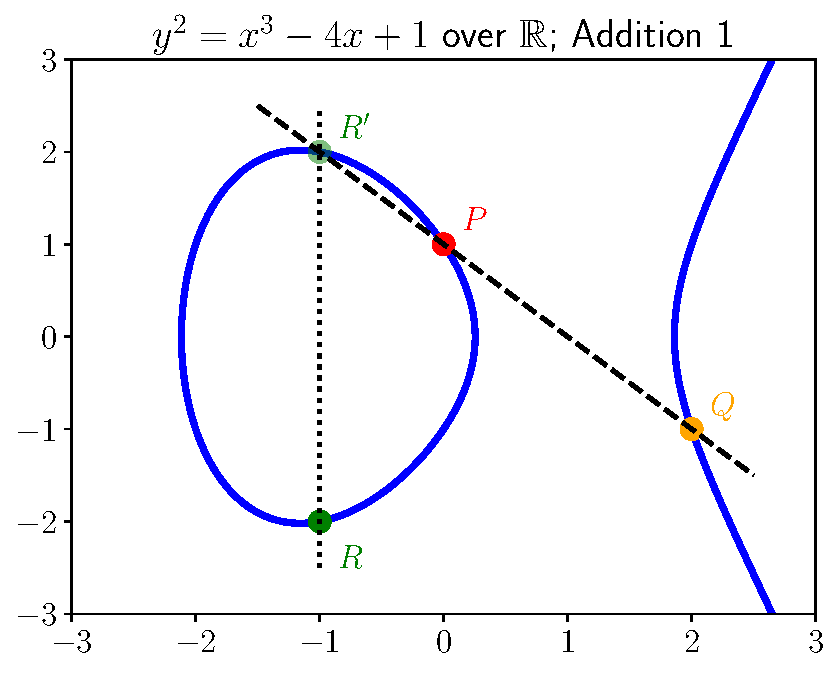
\includegraphics[width=0.70\textwidth]{plots/ec_reals/ec_reals_addition_1.pdf}
    \caption{Plot of elliptic curve addition over $\R$ for
        Example~\ref{example:ec_real_addition_1};
        this is an example of adding distinct points.
        We have
        $\textcolor{red}{P} + \textcolor{orange}{Q} =
        \textcolor[rgb]{0,0.33,0}{R}$.
        This figure shows
        $\textcolor{red}{\parens{0,1}} + \textcolor{orange}{\parens{2,-1}}
        = \textcolor[rgb]{0,0.33,0}{\parens{-1,-2}}$.}
    \label{fig:ec_real_plots_addition_1}
    \end{subfigure}

    \begin{subfigure}[t]{\textwidth}
        \centering
    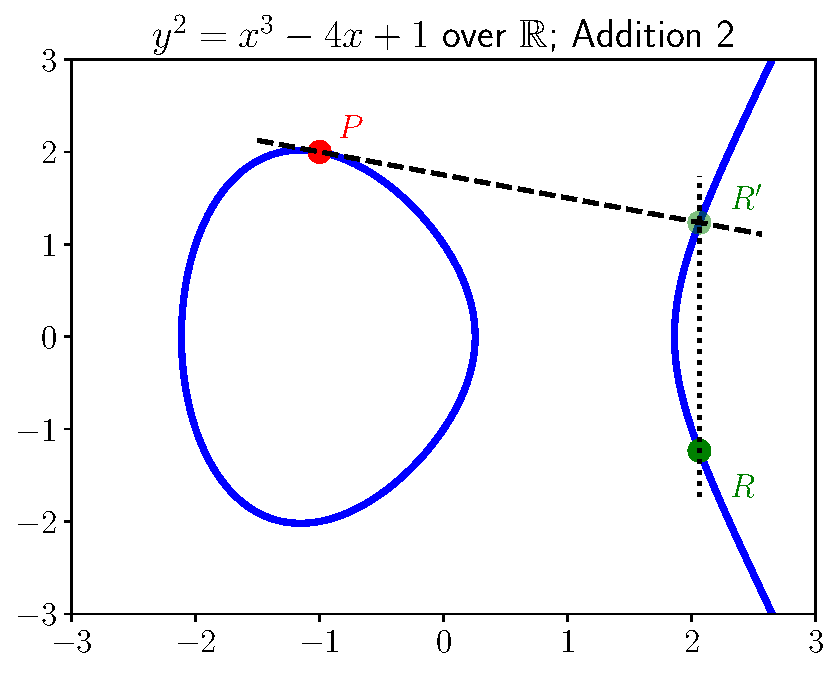
\includegraphics[width=0.70\textwidth]{plots/ec_reals/ec_reals_addition_2.pdf}
    \caption{Plot of elliptic curve addition over $\R$ for
        Example~\ref{example:ec_real_addition_2};
        this is an example of \emph{point doubling}.
        We have
        $\textcolor{red}{P} + \textcolor{red}{P} =
        \textcolor[rgb]{0,0.33,0}{R}$.
        This may also be written as
        $2\cdot\textcolor{red}{P} = \textcolor[rgb]{0,0.33,0}{R}$.
        This figure shows
        $2\cdot\textcolor{red}{\parens{-1,2}}
        = \textcolor[rgb]{0,0.33,0}{\parens{\frac{33}{16},-\frac{79}{64}}}$.}
    \label{fig:ec_real_plots_addition_2}
    \end{subfigure}

\caption[Plots of elliptic curve addition over the reals]{Here
    we plot elliptic curve addition over $\R$
    for Examples~\ref{example:ec_real_addition_1}
    and \ref{example:ec_real_addition_2}.
    Figure~\ref{fig:ec_real_plots_addition_1} shows the addition
    of distinct points while
    Figure~\ref{fig:ec_real_plots_addition_2} shows the addition
    of repeated points (point doubling).}
\label{fig:ec_real_plots_addition}
\end{figure}
